\documentclass[a4paper]{report}
\usepackage{microtype}
\usepackage{imakeidx}
\usepackage{hyperref}
\usepackage{color}
\usepackage{graphicx}
\usepackage{eso-pic}
\usepackage{multicol}
\usepackage{alltt}

\makeindex[intoc, columns=3]

\hypersetup{pdfauthor="Ravelli/Durex", pdftitle="durexForth: Operators Manual", colorlinks=true}
\begin{document}
\author{Ravelli/Durex}
\title{durexForth: Operators Manual}
% maketitle is necessary to populate html metadata.
\ifdef{\Css}{
  % This CSS mess creates a new set of columns at each heading.
  % In theory a (better!) effect could be achieved by moving the
  % heading out so it could span the columns.
  % The current variant has the heading in line with the top
  % of its group.
  % Ideally we'd break columns at page breaks, like print does.
  \Css{
    div.theindex {column-width: 9em; column-gap: 2em}
    p.theindex {column-span: all; column-width: 9em; column-gap: 2em}
    .index-item, .index-subitem, .index-subsubitem {display: block flex; justify-content: space-between; margin-top:0.2em}
  }
  \maketitle
}

\pagestyle{empty} % No page number on first page!
\AddToShipoutPicture*{
	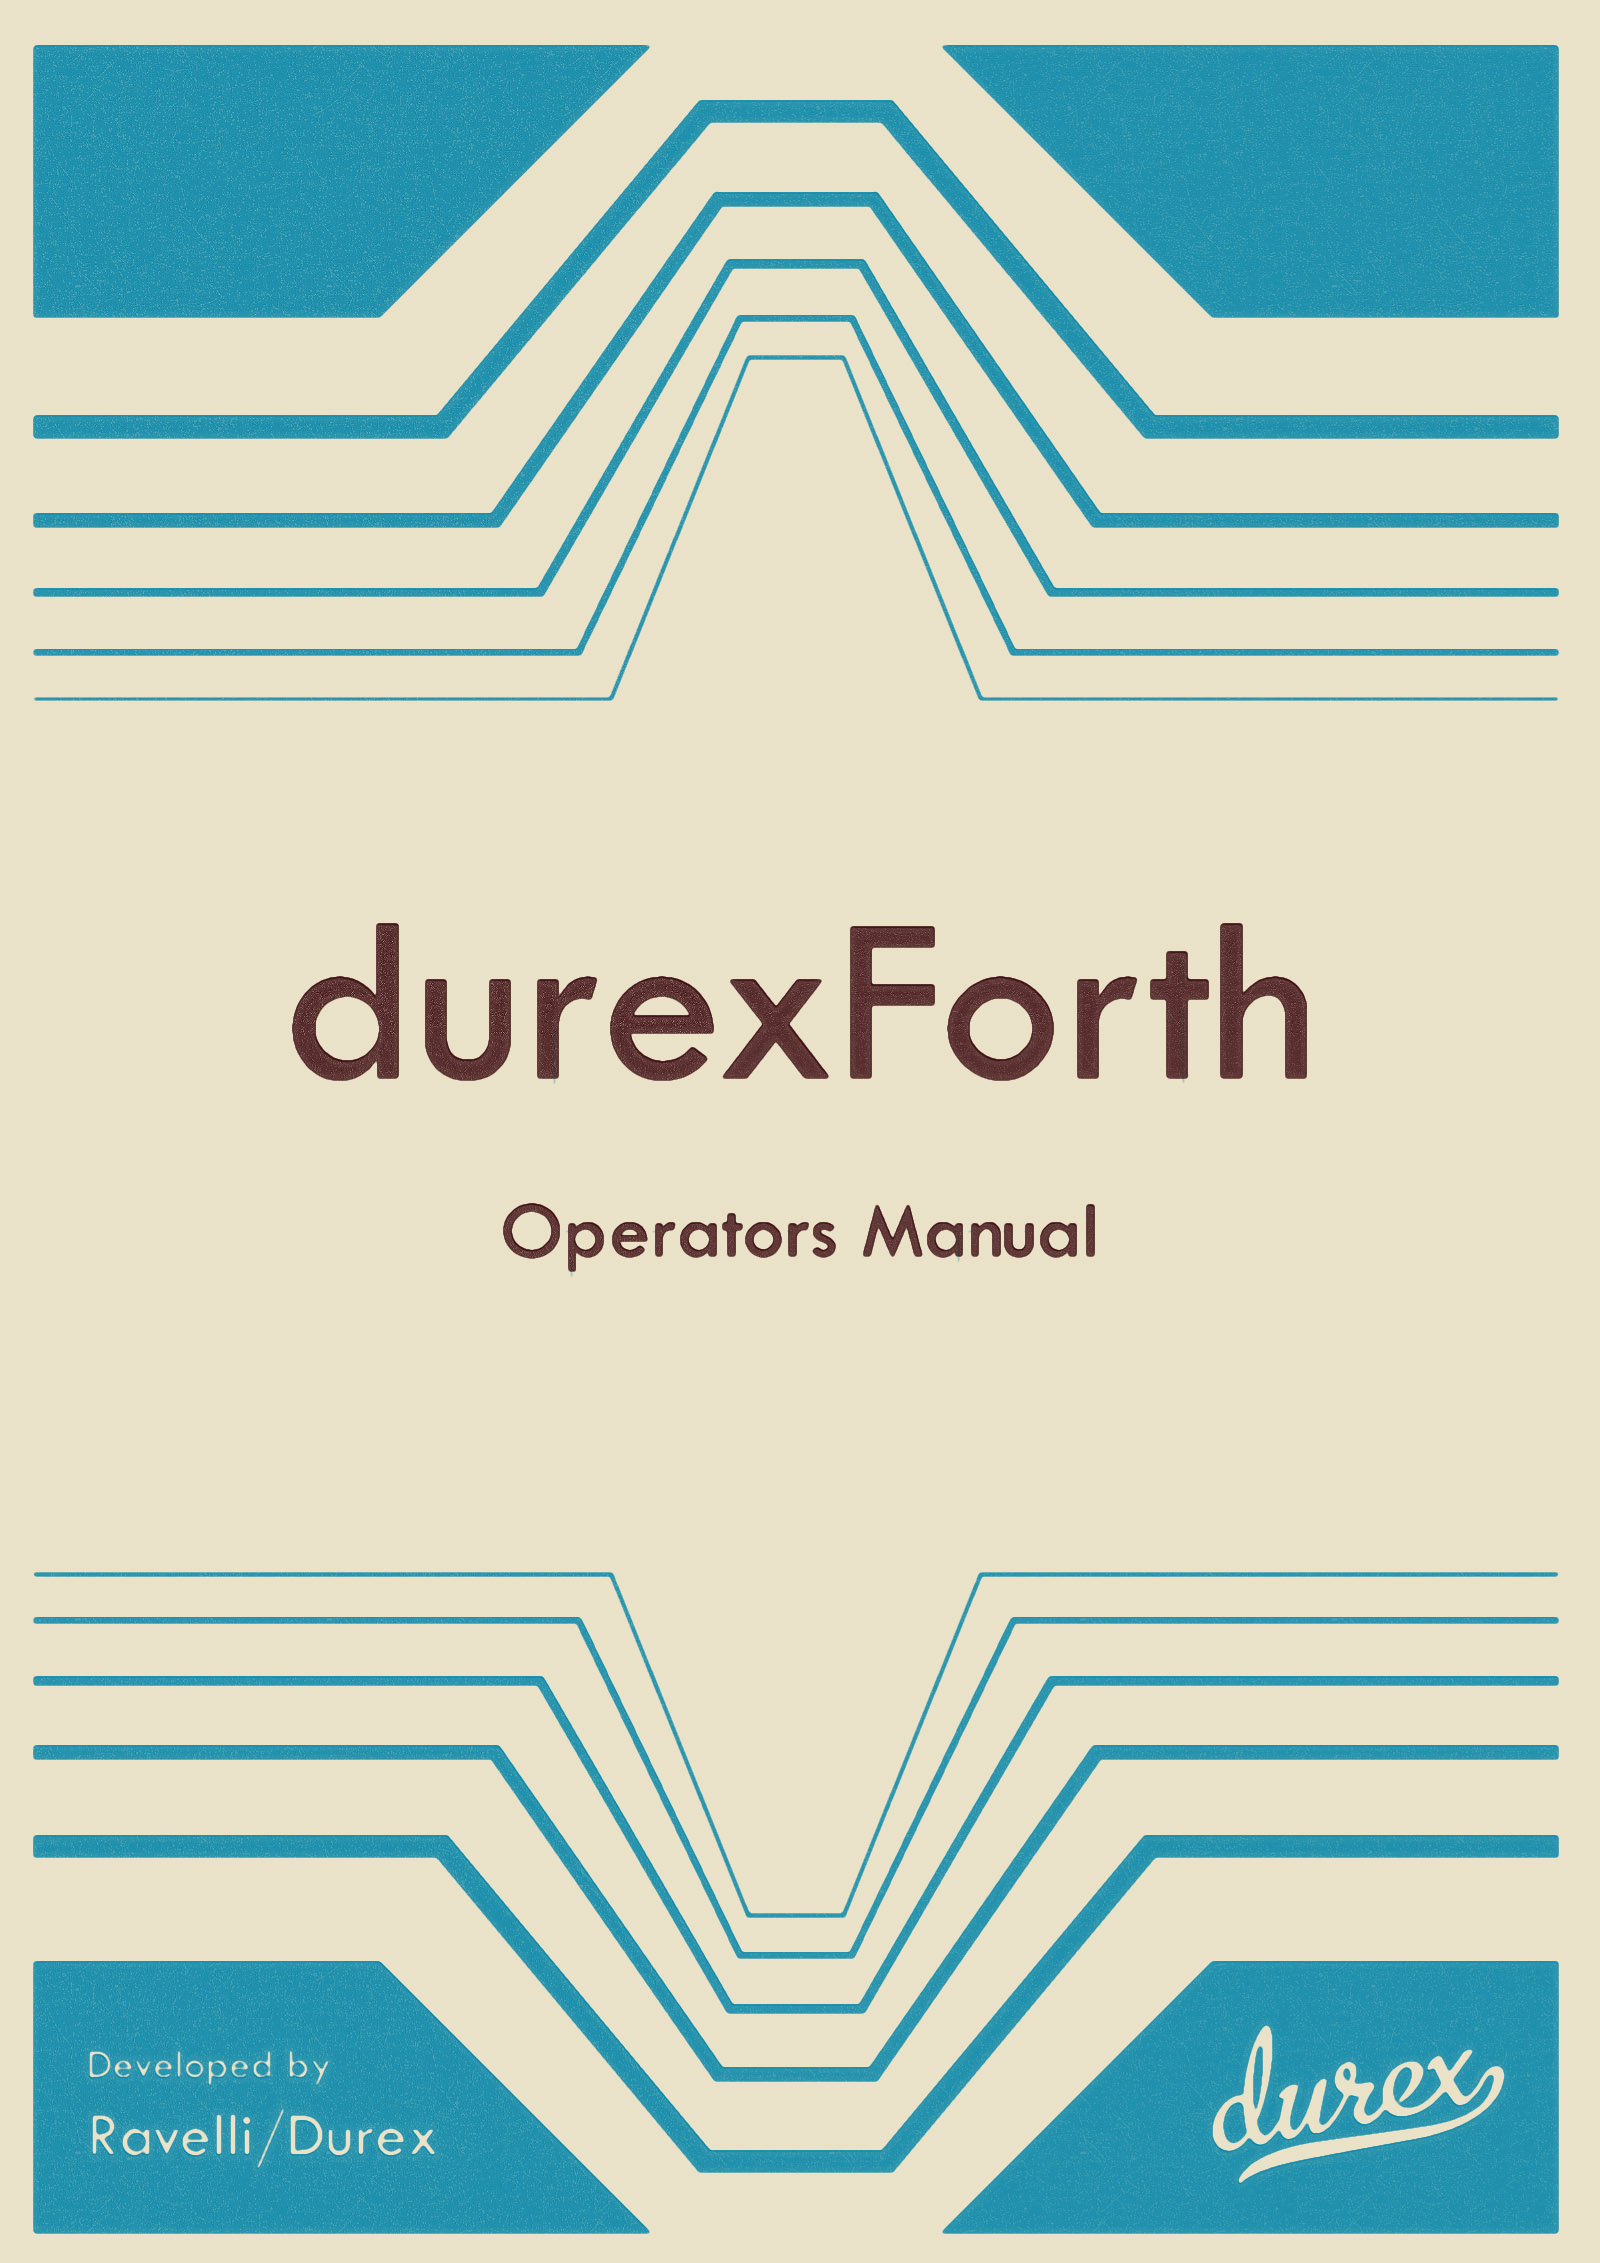
\includegraphics[width=21cm]{cover/durexForth-Vintage1.jpg}
}
\phantom{Invisible, but important}
\newpage
\pagestyle{plain}

\input{params-g.tex}

\setlength{\parindent}{0pt}

Release \texttt{\revisiontagdoc}, \space \revisiondate\\[18pt]

The MIT License\\

Copyright (c) 2008 \space Johan Kotlinski, Mats Andren

\begin{flushleft}
Permission is hereby granted, free of charge, to any person obtaining a copy
of this software and associated documentation files (the ``Software"), to deal
in the Software without restriction, including without limitation the rights
to use, copy, modify, merge, publish, distribute, sublicense, and/or sell
copies of the Software, and to permit persons to whom the Software is
furnished to do so, subject to the following conditions:
\end{flushleft}

\begin{flushleft}
The above copyright notice and this permission notice shall be included in
all copies or substantial portions of the Software.
\end{flushleft}

\begin{flushleft}
THE SOFTWARE IS PROVIDED ``AS IS", WITHOUT WARRANTY OF ANY KIND, EXPRESS OR
IMPLIED, INCLUDING BUT NOT LIMITED TO THE WARRANTIES OF MERCHANTABILITY,
FITNESS FOR A PARTICULAR PURPOSE AND NONINFRINGEMENT. IN NO EVENT SHALL THE
AUTHORS OR COPYRIGHT HOLDERS BE LIABLE FOR ANY CLAIM, DAMAGES OR OTHER
LIABILITY, WHETHER IN AN ACTION OF CONTRACT, TORT OR OTHERWISE, ARISING FROM,
OUT OF OR IN CONNECTION WITH THE SOFTWARE OR THE USE OR OTHER DEALINGS IN
THE SOFTWARE.
\end{flushleft}



\tableofcontents

\chapter{Introduction}

\section{Forth, the Language}

\subsection{Why Forth?}

Forth is a different language. It is old, a little weird and makes you think different.

What is cool about it? It is a very low-level and minimal language that has a few rough edges. At the same time, it is easy to make it a very high-level and domain-specific language, much like Lisp. 

Compared to C64 Basic, Forth is more attractive in almost every way. It is a lot more fast, memory effective and powerful.

Compared to C, specifically cc65, the story is a little different. It's hard to make a fair comparison. Theoretically Forth code can be very memory efficient, and it's possible to make Forth code that is leaner than C code. But it is also true that cc65 code is generally faster than Forth code.

The main advantage of Forth is that the environment runs on the actual machine. It would not be a
lot of fun to use a C compiler that runs on a standard C64. But with Forth, it's possible to create an entire development suite with editor, compiler and assembler that runs entirely on the C64.

Another advantage is that Forth has an interpreter. Compared to cross-compiling, it is really nice
to make small edits and tweaks without going through the entire edit-compile-link-transfer-boot-run cycle.

For a Forth introduction, please refer to the excellent
\href{http://www.forth.com/starting-forth/}{Starting Forth} by Leo Brodie. As a follow-up, I
recommend \href{http://thinking-forth.sourceforge.net/}{Thinking Forth} by the same author.

\subsection{Comparing to other Forths}

There are other Forths for c64, most notably Blazin' Forth. Blazin' Forth is excellent, but durexForth has some advantages:

\begin{itemize}
\item Store your Forth sources as text files - no crazy block file system.
\item durexForth is smaller.
\item The editor is a vi clone.
\item durexForth is open source (available at \href{http://code.google.com/p/durexforth/}{Google Code}).
\end{itemize}

\section{Appetizers}

Some demonstration files are included as appetizers.

\subsection{Graphics}

The gfxdemo package demonstrates the high-resolution graphics, with some examples adapted from the book "Step-By-Step Programming C64 Graphics" by Phil Cornes. 
Show the demos by entering:

\texttt{s" gfxdemo" load gfxdemo}

When a demo has finished drawing, press any key to continue.

\subsection{Fractals}

The fractal package demonstrates turtle graphics. You can load the package as follows:

\texttt{s" fractal" load}

The fractals can then be shown by typing \texttt{koch weed1 bush1 bush2}. When a fractal have finished drawing, press any key to continue.


\chapter{Tutorial}

\section{Interpreter}

Start up durexForth. If loaded successfully, it will greet you with a friendly \texttt{ok}. You have landed in the interpreter!

Let's warm it up a little. Enter \texttt{1} (followed by return). You have now put a digit on the stack. This can be verified by the command \texttt{.s}, which will print out the stack. Now enter \texttt{.} to pop the digit and print it to screen, followed by \texttt{.s} to verify that the stack is empty.

Now some arithmetics. \texttt{1000 a * .} will calculate $\$a \times \$1000$ and print the result on the screen. \texttt{6502 100 / 1- .} will calculate and print $(\$6502 / \$100) - 1$.

Let's define a word \texttt{bg!} for setting the border color\ldots 

\begin{verbatim}
: bg! d020 c! ;
\end{verbatim}

Now try entering \texttt{1 bg!} to change the border color to white.
Then, try changing it back again with \texttt{0 bg!}.

\section{Editor}

The editor (fully described in chapter \ref{editor}) is convenient for editing larger pieces of code. With it, you keep an entire source file loaded in RAM, and you can recompile and test it easily.

Start the editor by typing \texttt{vi}. You will enter the pink editor screen.

To enter text, first press \texttt{i} to enter insert mode. This mode allows you to insert text into the buffer. You can see that it's active on the \texttt{I} that appears in the lower left corner.

This is a good start for making a program. 
But first, let's get rid of the "bg!" word we created previously. Enter:

\begin{verbatim}
forget bg!
\end{verbatim}

\ldots and press $\leftarrow$ to leave insert mode. The line you entered forgets the \texttt{bg!} word that you defined in the last section, and everything defined after it. Let's try out if it works.

First, quit the editor by pressing \texttt{:q}. You should now be back in the interpreter screen.
Verify that the word \texttt{bg!} still exists by  entering \texttt{0 bg!}, \texttt{1 bg!} like you did
before. Then, jump back to the editor using the command \texttt{vi}. You should return to your edit buffer with the lonely \texttt{forget bg!} line.

Now, compile and run the buffer by pressing \texttt{F7}. You will be thrown out to the interpreter
again. Entering \texttt{bg!} should now give you the error \colorbox{yellow}{\texttt{bg!?}}. Success
--- we have forgotten the \texttt{bg!} word. Now, get back into the editor by entering \texttt{vi}.

Beneath \texttt{forget bg!}, add the following lines:

\begin{verbatim}
: flash d020 c@ 1+ d020 c! recurse ;
flash
\end{verbatim}

\texttt{flash} will cycle the border color infinitely. Before trying it out, go up and change \texttt{forget bg!} to \texttt{forget flash}. This makes sure you won't run out of RAM, no matter how many times you recompile the program. Now press \texttt{F7} to compile and run. If everything is entered right, you will be facing a wonderful color cycle.

To get back into the editor, press Restore key. Let's see how we can factor the program to get something more Forth'y:

\begin{verbatim}
forget bg
: bg d020 ; # border color addr
: inc dup c@ 1+ swap c! ; ( addr -- )
: flash bg inc recurse ;
flash
\end{verbatim}

(Note: Parentheses are used for multi-line comments or describing arguments and return values. \texttt{\#} is used for single-line comments.)

Of course, it is a matter of taste which version you prefer. Press \texttt{F7} to see if the new version runs faster or slower.

\section{Assembler}

If you need to flash as fast as possible, use the assembler:

\begin{verbatim}
:asm flash
here # push current addr
d020 inc,
jmp, # jump to pushed addr
;asm
flash
\end{verbatim}

\texttt{:asm} and \texttt{;asm} define a code word, just like \texttt{:} and \texttt{;} define Forth words. Within a code word, you can use assembler mnemonics. 

Note: As the x register contains the durexForth stack depth, it is important that it remains unchanged at the end of the code word.

\section{Console I/O Example}

This piece of code reads from keyboard and sends back the chars to screen:

\begin{verbatim}
: foo key emit recurse ;
foo
\end{verbatim}

\section{Avoiding Stack Crashes}

durexForth should be one of the fastest and leanest Forths for the C64. To achieve this, there are
not too many niceties for beginners. For example, compiled code has no checks for stack overflow
and underflow. This means that the system may crash if you do too many pops or pushes. This is not
much of a problem for an experienced Forth programmer, but until you reach that stage, handle the
stack with care.

\subsection{Commenting}

One helpful technique to avoid stack crashes is to add comments about stack usage.
In this example, we imagine a graphics word "drawbox" that draws a black box.
\texttt{( color -- )} indicates that it takes one argument on stack, and on exit it should
leave nothing on the stack. The comments inside the word indicate what the stack
looks like after the line has executed.

\begin{verbatim}
: drawbox ( color -- )
10 begin dup 20 < while # color x
10 begin dup 20 < while # color x y
2dup # color x y x y
4 pick # color x y x y color
blkcol # color x y
1+ repeat drop # color x
1+ repeat 2drop ;
\end{verbatim}

Once the word is working, it may be nice to again remove the \texttt{\#} comments as
they are no longer very interesting to read.

\subsection{Stack Checks}

Another useful technique during development is to check at the end of your main loop
that the stack depth is what you expect it to. This will catch stack underflows
and overflows.

\begin{verbatim}
: mainloop begin
# do stuff here...
depth if ." err" exit then
again ;
\end{verbatim}

\section{Configuring durexForth}

\subsection{Stripping Modules}

By default, durexForth boots up with all modules pre-compiled in RAM:

\begin{description}
\item[doloop] Do-loop words.
\item[debug] Words for debugging.
\item[asm] The assembler.
\item[vi] The text editor.
\item[ls] List disk contents.
\item[gfx] Graphics module.
\end{description}

To reduce RAM usage, you may make a stripped-down version of durexForth. Do this by following these steps:

\begin{enumerate}
\item Issue \texttt{forget modules} to forget all modules.
\item Optionally re-add the \texttt{modules} marker with \texttt{header modules}.
\item One by one, load the modules you want included with your new Forth. (E.g. \texttt{s" debug" load})
\item Save the new system with e.g. \texttt{s" acmeforth" save-forth}.
\end{enumerate}

\subsection{Custom Start-Up}

You may launch a word automatically at start-up by setting the variable \texttt{start} to the execution token of the word.  Example: \texttt{' megademo start !}

To save the new configuration to disk, use \texttt{save-forth}.

\section{How to Learn More}

\subsection{Internet Resources}

\subsubsection{Books and Papers}

\begin{itemize}
\item \href{http://www.forth.com/starting-forth/}{Starting Forth}
\item \href{http://thinking-forth.sourceforge.net/}{Thinking Forth}
\item \href{http://www.bradrodriguez.com/papers/}{Moving Forth: a series on writing Forth kernels}
\item \href{http://www.csbruce.com/~csbruce/cbm/transactor/v7/i5/p058.html}{Blazin' Forth --- An inside look at the Blazin' Forth compiler}
\item \href{http://www.drdobbs.com/architecture-and-design/the-evolution-of-forth-an-unusual-langua/228700557}{The Evolution of FORTH, an unusual language}
\item \href{http://galileo.phys.virginia.edu/classes/551.jvn.fall01/primer.htm}{A Beginner's Guide to Forth}
\end{itemize}

\subsubsection{Other Forths}

\begin{itemize}
\item \href{http://www.colorforth.com/cf.html}{colorForth}
\item \href{http://www.annexia.org/forth}{JONESFORTH}
\item \href{http://colorforthray.info/}{colorForthRay.info --- How\_to: with Ray St. Marie}
\end{itemize}

\subsection{Other}

\begin{itemize}
\item \href{http://code.google.com/p/durexforth/}{durexForth source code}
\end{itemize}

\chapter{Editor} \label{editor}

The editor is a vi clone. Launch it by entering \texttt{v foo} in the interpreter (\texttt{foo} being the file you want to edit). You may also enter \texttt{v} without argument to create an unnamed buffer. For more info about vi style editing, see \href{http://www.vim.org}{the Vim web site}.

The position of the editor buffer is \$7000.

\section{Key Presses}

\subsection{Inserting Text}
At startup, the editor is in command mode. The following commands enter insert mode, which allows you to enter text into the editor buffer. You can return to command mode with $\leftarrow$.
\begin{description}
\item[i] Insert text.
\item[R] Replace text.
\item[a] Append text.
\item[A] Append text at end of line.
\item[C] Change rest of line.
\item[S] Substitute line.
\item[s] Substitute character.
\item[o] Open new line after cursor line.
\item[O] Open new line on cursor line.
\item[cw] Change word.
\end{description}

\subsection{Navigation}
\begin{description}
\item[hjkl] Cursor left, down, up, right.
\item[Cursor Keys] ...also work fine.
\item[-] Scroll 1 line up.
\item[+] Scroll 1 line down.
\item[Ctrl+u] Half page up.
\item[Ctrl+d] Half page down.
\item[b] Go to previous word.
\item[w] Go to next word.
\item[e] Go to end of word.
\item[fx] Find char \texttt{x} forward.
\item[Fx] Find char \texttt{x} backward.
\item[0 | Home] Go to line start.
\item[\$] Go to line end.
\item[g] Go to start of file.
\item[G] Go to end of file.
\item[H] Go to home window line.
\item[L] Go to last window line.
\item[M] Go to middle window line.
\item[/\{string\}] Search forward for the next occurrence of the string.
\item[*] Search forward for the next occurrence of the word under the cursor.
\item[n] Repeat the latest search.
\end{description}

\subsection{Saving \& Quitting}

After quitting, the editor can be re-opened by entering \texttt{v}, and it will resume operations with the edit buffer preserved.

\begin{description}
\item[ZZ] Save and exit.
\item[:q] Exit.
\item[:w] Save. (Must be followed by return.)
\item[:w!filename] Save as.
\item[F7] Compile and run editor contents. Press Restore key to return to editor.
\end{description}

\subsection{Text Manipulation}
\begin{description}
\item[r] Replace character under cursor.
\item[x] Delete character.
\item[X] Backspace-delete character.
\item[dw] Delete word.
\item[dd] Cut line.
\item[D] Delete rest of line.
\item[yy] Yank (copy) line.
\item[p] Paste line below cursor position.
\item[P] Paste line on cursor position.
\item[J] Join lines.
\end{description}

\chapter{Forth Words}

\section{Stack Manipulation}

\begin{description}

\item[\index{drop}drop ( a -- )] Drop top of stack.
\item[\index{dup}dup ( a -- a a )] Duplicate top of stack.
\item[\index{swap}swap ( a b -- b a )] Swap top stack elements.
\item[\index{over}over ( a b -- a b a )] Make a copy of the second item and push it on top.
\item[\index{rot}rot ( a b c -- b c a )] Rotate the third item to the top.
\item[\index{-rot}-rot ( a b c -- c a b )] rot rot
\item[\index{2drop}2drop ( a b -- )] Drop two topmost stack elements.
\item[\index{2dup}2dup ( a b -- a b a b )] Duplicate two topmost stack elements.
\item[\index{?dup}?dup ( a -- a a? )] Dup a if a differs from 0.
\item[\index{nip}nip ( a b -- b )] swap drop
\item[\index{tuck}tuck ( a b -- b a b )] dup -rot
\item[\index{pick}pick ( $x_u$ ... $x_1$ $x_0$ $u$ -- $x_u$ ... $x_1$ $x_0$ $x_u$ )]
Pick from stack element with depth u to top of stack.
\item[\index{$>$r}$>$r ( a -- )] Move value from top of parameter stack to top of return stack.
\item[\index{r$>$}r$>$ ( -- a )] Move value from top of return stack to top of parameter stack.
\item[\index{r"@}r@ ( -- a )] Copy value from top of return stack to top of parameter stack.
\item[\index{depth}depth ( -- n)] \texttt{n} is the number of single-cell values contained in the data stack before \texttt{n} was placed on the stack.

\item[\index{lsb}lsb ( -- addr)] The top address of the LSB parameter stack.
\item[\index{msb}msb ( -- addr)] The top address of the MSB parameter stack.

\end{description}

\section{Utility}

\begin{description}
\item[\index{.}. ( n -- )] Prints top value of stack as signed number.
\item[\index{u.}u. ( u -- )] Prints top value of stack as unsigned number.
\item[\index{.s}.s] See stack contents.
\item[\index{emit}emit ( a -- )] Prints top value of stack as a PETSCII character. Example: \texttt{'q' emit}
\item[\index{\pounds}\pounds] Comment to end of line. (Used on C64/PETSCII.)
\item[\index{\textbackslash}\textbackslash] Comment to end of line. (Used when cross-compiling from PC/ASCII.)
\item[\index{(}(] Multiline comment. Ignores everything until a ).
\item[\index{bl}bl ( -- char )] Gives the PETSCII character for a space.
\item[\index{space}space] Displays one space.
\item[\index{spaces}spaces ( n -- )] Displays n spaces.
\item[\index{page}page] Clears the screen.
\item[\index{rvs}rvs] Reverse screen output.
\end{description}

\section{Mathematics}

\begin{description}
\item[\index{1+}1+ ( a -- b )] Increase top of stack value by 1.
\item[\index{1-}1- ( a -- b )] Decrease top of stack value by 1.
\item[\index{2+}2+ ( a -- b )] Increase top of stack value by 2.
\item[\index{2*}2* ( a -- b )] Multiply top of stack value by 2.
\item[\index{2/}2/ ( a -- b )] Divide top of stack value by 2.
\item[\index{100/}100/ ( a -- b )] Divides top of stack value by \$100.
\item[\index{+"!}+! ( n a -- )] Add n to memory address a.
\item[\index{+}+ ( a b -- c )] Add a and b.
\item[\index{-}- ( a b -- c )] Subtract b from a.
\item[\index{*}* ( a b -- c )] Multiply a with b.
\item[\index{/}/ ( a b -- q )] Divide a with b using floored division.
\item[\index{/mod}/mod ( a b -- r q )] Divide a with b, giving remainder r and quotient q.
\item[\index{mod}mod ( a b -- r )] Remainder of a divided by b.
\item[\index{*/}*/ ( a b c -- q )] Multiply a with b, then divide by c, using a 32-bit intermediary.
\item[\index{*/mod}*/mod ( a b c -- r q )] Like */, but also keeping remainder r.
\item[\index{0$<$}0$<$ ( a -- b )] Is a negative?
\item[\index{negate}negate ( a -- b )] Negates a.
\item[\index{abs}abs ( a -- b )] Gives absolute value of a.
\item[\index{min}min ( a b -- c )] Gives the lesser of a and b.
\item[\index{max}max ( a b -- c )] Gives the greater of a and b.
\item[\index{within}within ( n lo hi -- flag )] Returns true if lo $<=$ n $<$ hi.
\item[\index{$<$}$<$ ( n1 n2 -- flag )] Is n1 less than n2? (Signed.)
\item[\index{$>$}$>$ ( n1 n2 -- flag )] Is n1 greater than n2? (Signed.)
\item[\index{u$<$}u$<$ ( u1 u2 -- flag )] Is u1 less than u2? (Unsigned.)
\item[\index{u$>$}u$>$ ( u1 u2 -- flag )] Is u1 greater than u2? (Unsigned.)
\item[\index{lshift}lshift ( a b -- c )] Binary shift a left by b.
\item[\index{rshift}rshift ( a b -- c )] Binary shift a right by b.
\item[\index{base}base (variable)] Points to the cell that holds the numerical base.
\item[\index{decimal}decimal] Sets the numerical base to 10.
\item[\index{hex}hex] Sets the numerical base to 16.

\end{description}

\section{Double}

The following words use double-cell integers. On the stack, the cell containing the most significant part of a double-cell integer is above the cell containing the least significant part.

\begin{description}
\item[\index{dabs}dabs ( d -- ud )] Produces the absolute value of d.
\item[\index{dnegate}dnegate ( d -- d )] Negates the double-cell integer d.
\item[\index{s$>$d}s$>$d ( n -- d )] Converts the number n to the double-cell number d.
\item[\index{m"+}m+ ( d n -- d )] Add n to double-cell number d.
\item[\index{m*}m* ( a b -- d )] Multiply a with b, producing a double-cell value.
\item[\index{um*}um* ( a b -- ud )] Multiply a with b, giving the unsigned double-cell number ud.
\item[\index{um/mod}um/mod ( ud n -- r q )] Divide double-cell number ud by n, giving remainder r and quotient q. Values are unsigned.
\item[\index{fm/mod}fm/mod ( d n -- r q )] Divide double-cell number d by n, giving the floored quotient q and the remainder r. Values are signed.
\end{description}

\section{Logic}

\begin{description}
\item[\index{0=}0= ( a -- flag)] Is a equal to zero?
\item[\index{0$<>$}0$<>$ ( a -- flag )] Is a not equal to 0?
\item[\index{=}= ( a b -- flag )] Is a equal to b?
\item[\index{$<>$}$<>$ ( a b -- flag )] Does a differ from b?
\item[\index{and}and ( a b -- c )] Binary and.
\item[\index{or}or ( a b -- c )] Binary or.
\item[\index{xor}xor ( a b -- c )] Binary exclusive or.
\item[\index{invert}invert ( a -- b )] Flip all bits of a.
\end{description}

\section{Memory}

\begin{description}
\item[\index{"!}! ( value address -- )] Store 16-bit value at address.
\item[\index{"@}@ ( address -- value )] Fetch 16-bit value from address.
\item[\index{c"!}c! ( value address -- )] Store 8-bit value at address.
\item[\index{c"@}c@ ( address -- value )] Fetch 8-bit value from address.
\item[\index{fill}fill ( addr len char -- )] Fill range [addr, len + addr) with char.
\item[\index{move}move ( src dst len -- )]
Copies a region of memory \texttt{len} bytes long, starting at \texttt{src}, to emory beginning at \texttt{dst}.

\end{description}
\section{Compiling}

\begin{description}
\item[\index{:}: (C: "$<$spaces$>$name" -- )] Define the word with the given name and enter compilation state.
\item[\index{:noname}:noname ( -- xt )] Create an execution token and enter compilation state.
\item[\index{;}; ( -- ) ] End the current definition, allow it to be found in the dictionary and go back to interpretation state.
\item[\index{code}code ( "$<$spaces$>$name" -- )] Start assembling a new word.
\item[\index{;code};code] End assembler.
\item[\index{,}, ( n -- )] Write word on stack to \texttt{here} position and increase \texttt{here} by 2.
\item[\index{c,}c, ( n -- )] Write byte on stack to \texttt{here} position and increase \texttt{here} by 1.
\item[\index{allot}allot ( n -- )] Add n bytes to the body of the most recently defined word.
\item[\index{literal}literal ( n -- )] Compile a value from the stack as a literal value. Typical use: \texttt{: x ... [ a b * ] literal ... ;}
\index{{[char]}}\item[[char{]} c] Compile character \texttt{c} as a literal value.
\index{{[}}\item[[ ( -- )] Leave compile mode. Execute the following words immediately instead of compiling them.
\index{{]}}\item[{]} ( -- )] Return to compile mode.
\item[\index{immediate}immediate] Mark the most recently defined word as immediate (i.e. inside colon definitions, it will be executed immediately instead of compiled).
\index{{[']}}\item[{[']} name ( -- xt )] Place name's execution token xt on the stack. The execution token returned by the compiled phrase \texttt{['] x} is the same value returned by \texttt{' x} outside of compilation state. Typical use: \texttt{: x ... {[}'{]} name ... ;}
\item[\index{compile,}compile, ( xt -- )] Append \texttt{jsr xt} to the word being compiled. Typical use: \texttt{: recurse immed latest >xt compile, ;}
\item[\index{postpone}postpone xxx] Compile the compilation semantics (instead of interpretation semantics) of xxx. Typical use:
\begin{verbatim}
: endif postpone then ; immediate
: x ... if ... endif ... ;
\end{verbatim}
\item[\index{header}header xxx] Create a dictionary header with name \texttt{xxx}.
\item[\index{create}create xxx/does$>$] Create a word creating word \texttt{xxx} with custom behavior
specified after \texttt{does$>$}. For further description, see "Starting Forth."
\item[\index{state}state ( -- addr)] addr is the address of a cell containing the compilation-state flag. It is 1 when compiling, otherwise 0.
\end{description}

\section{Word List}

\begin{description}

\item[\index{hide}hide xxx] Removes \texttt{xxx} from the word list, while leaving its definition in place.
\item[\index{define}define ( "name" -- ) ] Assign \texttt{here} as the execution token of word \texttt{name} and enter the compilation state.
\item[\index{defcode}defcode ( "name" -- ) ] Like \texttt{define}, but starts a \texttt{code} segment instead.

\end{description}

\section{Variables}

\subsection{Values}

Values are fast to read, slow to write. Use values for variables
that are rarely changed.

\begin{description}
\item[\index{value}1 value foo] Create value foo and set it to 1.
\item[\index{constant}2 constant bar] Create constant value bar and set it to 2.
\item[foo] Fetch value of foo.
\item[\index{to}0 to foo] Set foo to 0.
\end{description}

\subsection{Variables}

Variables are faster to write to than values.

\begin{description}
\item[\index{variable}variable bar] Define variable bar.
\item[\index{"@}bar @] Fetch value of bar.
\item[\index{"!}1 bar !] Set bar to 1.
\end{description}

\section{Control Flow}

Control functions only work in compile mode, not in interpreter.

\begin{description}
\index{if}\item[\index{then}if ... then]

condition IF true-part THEN rest

\item[\index{else}if ... else ... then]

condition IF true-part ELSE false-part THEN rest

\index{do}\item[\index{loop}do ... loop] Start a loop with index \texttt{i} and limit. Example:

\begin{verbatim}
: print0to7 8 0 do i . loop ;
\end{verbatim}

\item[\index{+loop}do ... +loop] Start a loop with a custom increment. Example:

\begin{verbatim}
( prints odd numbers from 1 to n )
: printoddnumbers (n -- ) 1 do i . 2 +loop ;
\end{verbatim}

\index{i}\item[\index{j}i, j] Variables are to be used inside \texttt{do} .. \texttt{loop} constructs.
\texttt{i} gives inner loop index, \texttt{j} gives outer loop index.

\item[\index{leave}leave] Leaves the innermost loop.

\item[\index{unloop}unloop] Discards the loop-control parameters. Allows clean \texttt{exit} from within a loop.

\begin{verbatim}
: xx 0 0 do unloop exit loop ;
\end{verbatim}

\item[\index{begin}\index{again}begin ... again]

Infinite loop.

\item[\index{until}begin ... until]

BEGIN loop-part condition UNTIL.

Loop until condition is true.

\item[\index{while}\index{repeat}begin ... while ... repeat]

BEGIN condition WHILE loop-part REPEAT.

Repeat loop-part while condition is true.

\item[\index{exit}exit]

Exit function. Typical use: \texttt{: X test IF EXIT THEN ... ;}

\item[\index{recurse}recurse] Jump to the start of the word being compiled.

\item[\index{case}\index{endcase}case ... endcase, \index{of}of ... \index{endof}endof] Switch statements.

\begin{verbatim}
: tellno ( n -- )
case
1 of ." one" endof
2 of ." two" endof
3 of ." three" endof
." other"
endcase
\end{verbatim}

\end{description}

\section{Input}

\begin{description}

\item[\index{key}key ( -- c )] Gets one character from the keyboard.
\item[\index{key?}key? ( -- flag )] Returns true if a character is available for \texttt{key}.
\item[\index{getc}getc ( -- c )] Consumes the next character from the input buffer and increases \texttt{$>$in} by one. If no characters are available, the input buffer is refilled as needed.

\item[\index{char}char ( -- c )] Parses the next word, delimited by a space, and puts its first character on the stack.

\item[\index{$>$in}$>$in ( -- addr)] Gives the address of a cell containing the offset in characters from the start of the input buffer to the start of the parse area.

\item[\index{refill}refill ( -- )] Attempts to fill the input buffer from the input source.

\item[\index{source}source ( -- caddr u)] Gives the address of, and number of characters in, the input buffer.
\item[\index{source-id}source-id ( -- n )] Returns 0 if current input is keyboard, -1 if it is a string from \texttt{evaluate}, or the current file id.

\item[\index{word}word ( delim -- addr )] Reads a word from input, using delimiter \texttt{delim}, and puts the string address on the stack. If the delimiter is the space character, non-breaking space (hex a0) will also be treated as a delimiter.

\item[\index{parse-name}parse-name ( name -- caddr u )] Reads a word from input, delimited by whitespace. Skips leading spaces.

\item[\index{interpret}interpret ( -- value )] Interprets a word from input and puts it on the stack.

\item[\index{accept}accept ( addr u -- u )] Receive a string of at most u characters into the buffer that starts at addr. Returns how many characters were received.

\item[\index{evaluate}evaluate ( addr len -- )] Makes DurexForth evaluate the given string.

\item[\index{abort}abort] Empties the data stack and performs \texttt{quit}.

\item[\index{abort""}abort" ccc" ( f -- ) ] If \texttt{f} is true, print \texttt{ccc} and abort.

    Typical use: \texttt{: x ... test abort" error" ... ;}

\item[\index{quit}quit] Enters an endless loop where DurexForth interprets Forth commands from the keyboard. The word is named "quit" since it can be used to quit a program. It also does cleanup tasks like resetting I/O.

\end{description}

\section{Editing}

\begin{description}
\item[\index{v}v filename]

Opens text editor and starts editing the file named "filename".
If filename is empty and a buffer is already open, editor will pick up where it left.
Otherwise, an untitled buffer will be created.

\end{description}

\section{Strings}

\begin{description}
\item[\index{.(}.(]

Print a string. Example: \texttt{.( foo)}

\item[\index{.""}."]

Compile-time version of "\texttt{.(}". Example: \texttt{: foo ." bar" ;}

\item[\index{s""}s" ( -- caddr u )] Define a string. Compile-time only! Example: \texttt{s" foo"}.

\item[\index{count}count ( str -- caddr u )] Returns data address and length of the counted string str.

\item[\index{type}type ( caddr u -- )] Prints a string.

\item[\index{/string}/string ( caddr u n -- caddr+n u-n )] Adjusts the string by n characters.

\end{description}

\section{Number Formatting}

For more info about number formatting, read Starting Forth!

\begin{description}

\item[$<$\#]\index{$<$\#} Begins the number conversion process.
\item[\# ( ud -- ud )]\index{\#} Converts one digit and puts it in the start of the output string.
\item[\#s ( ud -- ud )]\index{\#s} Calls \# once, and repeats until the number is zero.
\item[\index{hold}hold ( ch -- )] Inserts the char at the start of the output string.
\item[\index{sign}sign ( a -- )] If \texttt{a} is negative, inserts a minus sign at the start of the output string.
\item[\#$>$ ( xd -- addr u )]\index{\#$>$} Drops xd and returns the output string.

\end{description}

\section{Vectored Execution}

\begin{description}
  % The ASCII/PETSCII ' character is replaced by TeX. \textquotesingle renders as one,
  % but then it eats the space next to it, and disappears from the index.
  % So, {} to prevent space eating and @ to customize index look.
\item[\index{'@\textquotesingle}\textquotesingle{} xxx ( -- addr )] Find execution token of word \texttt{xxx}.
\item[\index{find}find ( cstr -- cstr 0 $\vert$ xt -1 $\vert$ xt 1 )] Find the definition named in the counted string cstr. If the definition is not found, return cstr and 0, otherwise return the execution token. If the definition is immediate, also return 1, otherwise also return -1.
\item[\index{find-name}find-name ( caddr u -- 0 $\vert$ nt )] Get the name token (dictionary pointer) of word named in the string, or 0 if the word is not found.
\item[\index{execute}execute ( xt -- )] Execute the execution token on top of stack.
\item[\index{$>$xt}$>$xt ( addr -- xt )] Get execution token of word at adress \texttt{addr}.

\end{description}

\section{Debugging}

\begin{description}
\item[\index{words}words] List all defined words.
\item[\index{size}size] \texttt{size foo} prints size of \texttt{foo}.
\item[\index{dump}dump ( n -- )] Memory dump starting at address n.
\item[n] \index{n}Continue memory dump where last one stopped.
\item[\index{see}see name ( -- )] Decompiles and prints the named word. Works on colon definitions only. Optionally included with \texttt{include see}.
\end{description}

\section{System State}

\begin{description}


\item[\index{latest}latest (value)] Address of latest defined header.

\item[\index{here}here (value)] Write position of the Forth compiler (usually first unused byte of code space). Many C64 assemblers refer to this as program counter or \texttt{*}.

\item[\index{pad}pad ( -- addr )] Address of the \texttt{pad}, a 161-byte memory region that can be used freely by user words. No built-in words will modify this region.

\item[\index{marker}marker name ( -- )] Creates a word that when called, forgets itself and all words that were defined after it. Example:

\begin{verbatim}
marker forget
: x ;
forget
\end{verbatim}

\item[\index{dowords}dowords ( xt -- )] Remove \texttt{xt} from the stack. Execute \texttt{xt} once for every word in the wordlist, passing the name token \texttt{nt} of the word to \texttt{xt}, until the wordlist is exhausted or until \texttt{xt} returns false. The invoked \texttt{xt} has the stack effect \texttt{( k * x nt -- l * x flag)}. If \texttt{flag} is true, \texttt{dowords} will continue on to the next name, otherwise it will return.

\begin{verbatim}
\ from debug.fs
: (words) more name>string space 1 ;
: words ['] (words) dowords ;
\end{verbatim}
\end{description}

\section{Disk I/O}

\begin{description}
\item[\index{include}include filename ( -- )] Load and parse file. Example: \texttt{include test}
\item[\index{included}included ( filenameptr filenamelength -- )] Load and parse file.
\item[\index{require}require filename ( -- )] Like include, except that load is skipped if the file is already loaded.
\item[\index{required}required ( filenameptr filenamelength -- )] Like included, except that load is skipped if the file is already loaded.
\item[\index{loadb}loadb ( filenameptr filenamelength dst -- endaddr )] Load binary block to dst. Returns 0 on failure, otherwise address after last written byte.
\item[\index{saveb}saveb ( start end filenameptr filenamelength -- )] Save binary block.
\item[\index{device}device ( device\# -- )] Switches the active device.
\item[\index{save-forth}save-forth filename ( -- )] Saves the forth to the given filename.
\item[\index{ls}ls ( -- )] Load disk directory to here and display, with optional drive \# and wildcards. Example: \texttt{ls \$1:*=p} Load directory, drive 1 only prg files.
\item[\index{rdir}rdir ( addr -- )] Display disk directory previously loaded to addr.
\end{description}

\subsection{DOS Commands}

Words for sending DOS commands to drives and reading drive status are available by including \texttt{dos}.

\begin{description}
    \item[\index{send-cmd}send-cmd ( addr length -- )] Writes the given string to secondary address 15 on the current device, and prints the drive's response. The following example defines a word, \texttt{backup} that creates a copy of \texttt{durexforth} called \texttt{backup}:
    \begin{verbatim}
        : backup s" copy0:backup=durexforth" send-cmd ;
        backup
    \end{verbatim}

    \item[\index{dos}dos command ( -- )] Sends \texttt{command} to the current device's command channel, and prints the response. Note that the remainder of the line is treated as part of the command. This makes it possible to refer to file names that contain spaces, but means that \texttt{dos} and its command should be on their own line, or the last words on a line. Example: \texttt{dos scratch0:old file} will delete a file named ``\texttt{old file}''.
\end{description}

\subsection{Low-Level Device I/O}

For more advanced uses, words corresponding to the standard Commodore Kernal IO routines are available by including \texttt{io}.

\begin{description}
    \item[\index{open}open ( filenameptr filenamelength file\# secondary-addr -- ioresult )] Open a logical file.
    \item[\index{chkin}chkin ( file\# -- ioresult )] Use a logical file as input device.
    \item[\index{chkout}chkout ( file\# -- ioresult )] Use a logical file as output device.
    \item[\index{clrchn}clrchn ( -- )] Resets input and output to the keyboard and screen.
    \item[\index{close}close ( file\# -- )] Close a logical file.
    \item[\index{readst}readst ( -- status )] Returns the status of the last IO operation. For serial-bus devices, \texttt{\$01} = write timeout, \texttt{\$02} = read timeout, \texttt{\$40} = end of file (EOI), \texttt{\$80} = device not present.
    \item[\index{chrin}chrin ( -- char)] Reads a character from the current input device.
    \item[\index{ioabort}ioabort ( ioresult -- )] Handles error conditions for \texttt{open}, \texttt{chkin} and \texttt{chkout}. On failure, print error message and abort.
\end{description}

As per the underlying Kernal routines, \texttt{chrin} does not check for end-of-file or any other error condition. \texttt{readst} should be called to ensure that the returned character is valid.

The \texttt{ioresult} value returned by \texttt{open}, \texttt{chkin} and \texttt{chkout} is 0 on success, or a Kernal error number if an error occurred.

Note that use of low-level device I/O may interfere with disk accesses done by durexForth and the \texttt{V} editor. The following guidelines should be followed to avoid interference:

\begin{itemize}
    \item Avoid using file numbers 15 and below (remember, any number up to 127 can be used as a file number).
    \item Only use input/output redirection (\texttt{chkin} and \texttt{chkout}) within word definitions, and ensure that \texttt{clrchn} is called before exit.
    \item Close files as soon as they are no longer needed.
    \item If multiple files are open, always call \texttt{clrchn} to end any serial bus transactions before calling \texttt{open} or switching between files with \texttt{chkin} or \texttt{chkout}.
\end{itemize}

\section{Compatibility}

The \texttt{compat} module contains various words that are not deemed necessary for enjoyable DurexForth operation, but still must be provided to comply with the Forth 2012 core standard.

\begin{description}
    \item[\index{environment?}environment? ( addr u -- 0 )] Environmental query.
    \item[\index{cell+}cell+ ( n -- n+2 )] 2+
    \item[\index{cells}cells ( n -- n*2 )] 2*
    \item[\index{char+}char+ ( n -- n+1 )] 1+
    \item[\index{align}align ( -- )] No-op
    \item[\index{aligned}aligned ( -- )] No-op
    \item[\index{chars}chars ( -- )] No-op
    \item[\index{2"@}2@ ( address -- x1 x2 )] Fetch 32-bit value from address. x2 is stored at address, and x1 is stored at address + 2.
    \item[\index{2"!}2! ( x1 x2 address -- )] Store 32-bit value to address. x2 is stored at address, and x1 is stored at address + 2.
    \item[\index{2over}2over ( a b c d -- a b c d a b )] Copies cell pair a b to top of stack.
    \item[\index{2swap}2swap ( a b c d -- c d a b )] Exchanges the top two cell pairs.
    \item[\index{$>$number}$>$number ( ud addr u -- ud addr2 u2 )] Converts the string in \texttt{addr u} to digits, using \texttt{BASE}, and adds each digit into ud after multiplying it with \texttt{BASE}. \texttt{addr2 u2} contains the part of the string that was not converted.
    \item[\index{$>$body}$>$body ( xt -- addr )] Returns the data field address that belongs to the execution token. Example use: \texttt{' foo >body}
    \item[\index{sm/rem}sm/rem ( d n -- r q )] Divide double-cell number d by n, giving the symmetric quotient q and the remainder r. Values are signed.

\end{description}

\section{Kernel Calls}

Safe kernel calls may be done from Forth words using \texttt{sys} ( addr -- ). The helper variables \texttt{ar}, \texttt{xr}, \texttt{yr} and \texttt{sr} can be used to set arguments and get results through the a, x, y and status registers.

Example: \texttt{'0' ar c! \$ffd2 sys} calls the CHROUT routine, which prints \texttt{0} on screen.

\section{Turn-key Utilities}
These words are available by including \texttt{turnkey}.
\begin{description}
\item[\index{top}top ( -- addr )] Address of the top of the dictionary, default: \$9fff.

\item[\index{top"!}top! ( addr -- )] Relocates the dictionary to \texttt{addr}. Example:

\begin{verbatim}
\ not using $a000 block, give all memory to dictionary
$cbff top!
\end{verbatim}

\item[\index{save-pack}save-pack filename ( -- )] Saves a compact version of forth to the given filename.
\item[\index{save-prg}save-prg filename ( -- )] Saves a forth program with no dictionary to filename.
\end{description}

	Further details on use of these words outlined in the \hyperref[Turn-key Operation]{Turn-key Operation} section of the tutorial.

\chapter{Graphics}

As of durexForth v1.2, high-resolution graphics support is included.

\section{Turtle Graphics}

Turtle graphics are mostly known from LOGO, a 1970s programming language.
It enables control of a turtle that can move and turn while holding a pen.
The turtle graphics library is loaded with \texttt{include turtle}.

\begin{description}
\item[init ( -- )] Initializes turtle graphics.
\item[forward ( px -- )] Moves the turtle \texttt{px} pixels forward.
\item[back ( px -- )] Moves the turtle \texttt{px} pixels back.
\item[left ( deg -- )] Rotates the turtle \texttt{deg} degrees left.
\item[right ( deg -- )] Rotates the turtle \texttt{deg} degrees right.
\item[penup ( -- )] Pen up (disables drawing).
\item[pendown ( -- )] Pen down (enables drawing).
\end{description}

\section{High-Resolution Graphics}

The high-resolution graphics library is loaded with \texttt{include gfx}. 
It is inspired by "Step-by-Step Programming Commodore 64: Graphics Book 3."
Some demonstrations can be found in \texttt{gfxdemo}. 
\begin{description}
\item[hires ( -- )] Enters the high-resolution drawing mode.
\item[lores ( -- )] Switches back to low-resolution text mode.
\item[clrcol ( colors -- )] Clears the high-resolution display using \texttt{colors}. Colors is a
byte value with foreground color in high nibble, background color in low nibble. E.g. \texttt{15
clrcol} clears the screen with green background, white foreground.
\item[blkcol ( col row colors -- )] Changes colors of the 8x8 block at given position.
\item[plot ( x y -- )] Sets the pixel at x, y.
\item[peek ( x y -- p )] Gets the pixel at x, y.
\item[line ( x y -- )] Draws a line to x, y.
\item[circle ( x y r -- )] Draws a circle with radius r around x, y.
\item[erase ( mode -- )] Changes blit method for line drawing. \texttt{1 erase} uses \texttt{xor}
for line drawing, \texttt{0 erase} switches back to \texttt{or}.
\item[paint ( x y -- )] Paints the area at x, y.
\item[text ( column row str strlen -- )] Draws a text string at the given position. E.g. \texttt{10
8 parse-name hallo text} draws the message "hallo" at column 16, row 8.
\item[drawchar ( column row addr -- )] Draws a custom character at given column and row, using the 8 bytes long data starting at addr.
\end{description}

\chapter{SID}

\section{Introduction}

The \texttt{sid} module contains words for controlling the SID chip. To load it, type \texttt{include sid}. To test that it works, run \texttt{sid-demo}.

\subsection{Voice Control}

\begin{description}
    \item[voice! ( n -- )] Selects SID voice 0-2.
    \item[freq! ( n -- )] Writes 16-bit frequency.
    \item[pulse! ( n -- )] Writes 16-bit pulse value.
    \item[control! ( n -- )] Writes 8-bit control value.
    \item[srad! ( srad -- )] Writes 16-bit ADSR value. (Bytes are flipped.)
    \item[note! ( n -- )] Plays note in range [0, 94], where 0 equals C-0. The tuning is made for PAL.
\end{description}

\subsection{SID Control}

\begin{description}
    \item[cutoff! ( n -- )] Writes 16-bit filter cutoff value.
    \item[filter! ( n -- )] Writes 8-bit filter value.
    \item[volume! ( n -- )] Writes 8-bit volume.
\end{description}

\chapter{Music}

\section{Music Macro Language}

Music Macro Language (MML) has been used since the 1970s to sequence music on computer and video game systems. MML support is included in durexForth, starting with version 1.3. The package is loaded with \texttt{s" mml" load"}. Two demonstration songs can be found in the \texttt{mmldemo} package.

MML songs are played using the Forth word \texttt{play-mml} which takes three strings, one MML melody for each of the three SID voices. An example song is as follows:

\begin{verbatim}
: frere-jaques
s" o3l4fgaffgafab->c&c<ab->c&cl8cdc<b-l4af>l8cdc<b-l4affcf&ffcf&f"
s" r1o3l4fgaffgafab->c&c<ab->c&cl8cdc<b-l4af>l8cdc<b-l4affcf&ffcf&f"
s" " play-mml ;
\end{verbatim}

\section{Commands}

\begin{description}
\item[cdefgab] The letters \texttt{c} to \texttt{b} represent musical notes. Sharp notes are produced by appending a \texttt{+}, flat notes are produced by appending a \texttt{-}. The length of a note is specified by appending a number representing its length as a fraction of a whole note -- for example, \texttt{c8} represents a C eight note, and \texttt{f+2} an F\# half note. Valid note lengths are 1, 2, 3, 4, 6, 8, 16, 24 and 32. Appending a \texttt{.} increases the duration of the note by half of its value.
\item[o] Followed by a number, \texttt{o} selects the octave the instrument will play in.
\item[r] A rest. The length of the rest is specified in the same manner as the length of a note.
\item[$<$,$>$] Used to step down or up one octave.
\item[l] Followed by a number, specifies the default length used by notes or rests which do not explicitly specify one.
\item[\&] Ties two notes together.
\end{description}

\chapter{Assembler Mnemonics}

\begin{multicols}{5}{
\begin{verbatim}
adc,#
adc,
adc,x
adc,y
adc,(x)
adc,(y)

and,#
and,
and,x
and,y
and,(x)
and,(y)

asla,
asl,
asl,x

bcc,
bcs,
beq,

bit,

bmi,
bne,
bpl,
brk,
bvc,
bvs,
clc,
cld,
cli,
clv,

cmp,#
cmp,
cmp,x
cmp,y
cmp,(x)
cmp,(y)

cpx,#
cpx,

cpy,#
cpy,

dec,
dec,x

dex,
dey,

eor,#
eor,
eor,x
eor,y
eor,(x)
eor,(y)

inc,
inc,x

inx,
iny,

jmp,
jmp,()

jsr,

lda,#
lda,
lda,x
lda,y
lda,(x)
lda,(y)

ldx,#
ldx,
ldx,y

ldy,#
ldy,
ldy,x

lsra,
lsr,
lsr,x

nop,

ora,#
ora,
ora,x
ora,y
ora,(x)
ora,(y)

pha,
php,
pla,
plp,

rola,
rol,
rol,x

rora,
ror,
ror,x

rti,
rts,

sbc,#
sbc,
sbc,x
sbc,y
sbc,(x)
sbc,(y)

sec,
sed,
sei,

sta,
sta,x
sta,y
sta,(x)
sta,(y)

stx,
stx,y

sty,
sty,x

tax,
tay,
tsx,
txa,
txs,
tya,
\end{verbatim}
}
\end{multicols}

\appendix
\chapter{Assembler Mnemonics}

\begin{multicols}{5}{
\begin{verbatim}
adc,#
adc,
adc,x
adc,y
adc,(x)
adc,(y)

and,#
and,
and,x
and,y
and,(x)
and,(y)

asl,a
asl,
asl,x

bcc,
bcs,
beq,
bmi,
bne,
bpl,
bvc,
bvs,

bit,
brk,
clc,
cld,
cli,
clv,

cmp,#
cmp,
cmp,x
cmp,y
cmp,(x)
cmp,(y)

cpx,#
cpx,

cpy,#
cpy,

dec,
dec,x

dex,
dey,

eor,#
eor,
eor,x
eor,y
eor,(x)
eor,(y)

inc,
inc,x

inx,
iny,

jmp,
(jmp),

jsr,

lda,#
lda,
lda,x
lda,y
lda,(x)
lda,(y)

ldx,#
ldx,
ldx,y

ldy,#
ldy,
ldy,x

lsr,a
lsr,
lsr,x

nop,

ora,#
ora,
ora,x
ora,y
ora,(x)
ora,(y)

pha,
php,
pla,
plp,

rol,a
rol,
rol,x

ror,a
ror,
ror,x

rti,
rts,

sbc,#
sbc,
sbc,x
sbc,y
sbc,(x)
sbc,(y)

sec,
sed,
sei,

sta,
sta,x
sta,y
sta,(x)
sta,(y)

stx,
stx,y

sty,
sty,x

tax,
tay,
tsx,
txa,
txs,
tya,
\end{verbatim}
}
\end{multicols}

\chapter{Memory Map}

\begin{description}
\item[... - \$87] Parameter stack (grows downwards). Placing parameter stack here gives good performance, but it also means that BASIC Kernal cannot be used without extra precautions.
\item[\$88 - \$8d] Temporary storage for low-level Forth words.
\item[\$8e - \$8f] Instruction pointer.
\item[\ldots]
\item[\$801 - \texttt{here}] Forth Kernel followed by dictionary.
\item[\ldots]
\item[\texttt{bufstart} - \texttt{eof}] Editor space.
\end{description}


\chapter{Word Anatomy}

\section{Inspecting a Word}

Let us define a word and see what it gets compiled to.

\begin{verbatim}
: bg d020 c! ;
\end{verbatim}

When the word is defined, you can get its start address by \texttt{loc bg}, and the contents of bg can be dumped using \texttt{loc bg dump}. Try it, and you will get output like the following:

\begin{alltt}
48e7  a0 48 02 42 47 20 86 08 .h.bg ..
48ef  9c 10 20 d0 ae 0a ce 10 .. .....
48f7  ff ff ff ff ff ff ff ff ........
49ff  ...
\end{alltt}

Here, we can see that the "bg" word is 16 bytes long and starts at address \$48e7. It contains three parts: Header, code field and data field.

\section{Header}

\begin{alltt}
48e7  \textcolor{red}{a0 48 02 42 47} 20 86 08 \textcolor{red}{.h.bg} ..
48ef  9c 10 20 d0 ae 0a ce 10 .. .....
\end{alltt}

The first two bytes contain a back-pointer to the previous word, starting at \$48a0. The next byte, "02", is the length of "bg" name string. After that, the string "bg" follows. (42 = 'b', 47 = 'g')

The name length byte is also used to store special attributes of the word. Bit 7 is "immediate" flag, which means that the word should execute immediately instead of being compiled into word definitions. ("(" is such an example of an immediate word that does not get compiled.) Bit 6 is "hidden" flag, which makes a word unfindable. Since bg is neither immediate nor hidden, bits 7-6 are both clear.

\section{Code Field}

\begin{alltt}
48e7  a0 48 02 42 47 \textcolor{red}{20 86 08} .h.bg \textcolor{red}{..}
48ef  9c 10 20 d0 ae 0a ce 10 .. .....
\end{alltt}

The code field contains the 6502 instruction "jsr \$886". \$886 is the place of the DOCOL word, which is responsible for pushing the Forth instruction pointer (IP) to the return stack, and then making IP point to the data field of bg.

\section{Data Field}

\begin{alltt}
48e7  a0 48 02 42 47 20 86 08 .h.bg ..
48ef  \textcolor{red}{9c 10 20 d0 ae 0a ce 10 .. .....}
\end{alltt}

The data field contains a list of pointers to code fields to be executed by DurexForth. The first two bytes contain \$109c, the code field adress (CFA) of the \texttt{lit} word. \texttt{lit} is responsible for pushing the two following bytes (\$d020) to the parameter stack. After that, we find \$aae, the CFA of \texttt{c!}. Finally, \$10ce is the CFA of \texttt{exit}, which restores the instruction pointer that DOCOL previously pushed to the return stack.


\printindex
\end{document}
